% Question  ##################################################################################################################
\section{Question 3}\label{ssec:pt1q3}
\textbf{Under the assumption of Markov property, the Binomial tree provides a method of how the future
price of an instrument, can be modelled. By investigating the statistics of Google daily returns for the
last 5 years (till 31/12/2017), construct a binomial tree model that projects Google stock price for
the first 6 months of 2018, on a monthly basis.}

\noindent
\textbf{In your answers explain the method/steps used.}

% END Question  ##############################################################################################################

% Question (i) ###############################################################################################################

\subsection{Q3 (i)}\label{sssec:pt1q3i}
\textbf{Present the projected probability and stock price binomial trees.}

\noindent
Code used in this question can be found in ‘Question 3 (i)’ in the notebook. The Google prices downloaded in Q1 (vii) were reloaded and used for this task. After reloading the prices, the log return was computed for each row. The annualized returns and volatility were also computed assuming that a year has 250 days. Furthermore, the last closing price was referenced and saved in a variable, as this will be used as a parameter to compute the binomial tree. A function called ‘binomial\_tree’ was created in the ‘fintech’ library to construct such tree. This function is shown in Fig.~\ref{fig:binomial_1} and Fig.~\ref{fig:binomial_2}.

\noindent
First off to construct the binomial tree we need to compute the following variables; time step $(\frac{0.5}{6})$ since we have half a year and projecting for 6 months, Up Factor $(\exp(volatility \times \sqrt{time \ step}))$, Down Factor $(\frac{1}{Up \ Factor})$, Up Probability $(\frac{(\exp(return \times time \ step))}{(Up \ Factor - Down \ Factor)})$ and Down Probability $(1 - Up \ Probability)$. 

\noindent
After these variables are computed an empty 2D numpy array was initialized to hold the projected prices for the binomial tree. The first element (0,0) was set to the last closing price.  The function then loops for the number of time periods specified and computes the stock price binomial tree. After this iteration finishes, you will end up with a sparse matrix where half of the elements are empty, and the other half are filled with the prices. The symmetry between the prices and the empty values is diagonal. Fig.~\ref{fig:binomial_ex} better explains what is happening inside the for loop to compute the projected prices. Table.~\ref{tbl:binomial_prices} shows the output for this part of the function, which is the projected stock price binomial trees. 

\noindent
Similarly to the prices, another empty 2D numpy array was initialized to hold the projected probabilities. The first element (0,0) was set to 1 since this value corresponds to the last closing price. Again, this function loops for the number of time periods specified to compute the probabilities. The output is quite like the previous step as it is also outputs a sparse matrix, where half of the elements are empty, and the other half are filled the probabilities. The symmetry between the probabilities and the empty values is diagonal. Fig.~\ref{fig:binomial_ex2} better explains what is happening inside the for loop to compute the projected probabilities. Table.~\ref{tbl:binomial_probs} shows the output for this part of the function, which is the projected probability binomial trees.

\begin{figure}[H]
\centering
  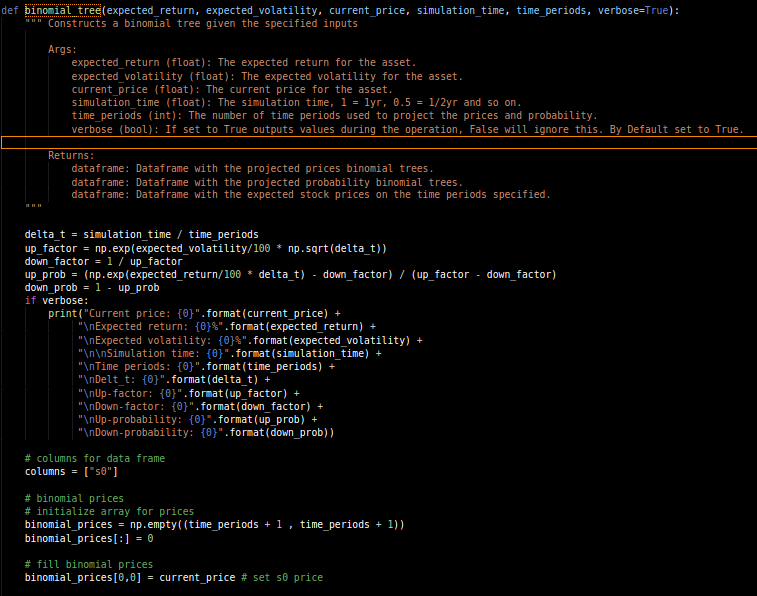
\includegraphics[scale = .62]{imgs/binomial_tree_1.png}
  \caption{Function to construct Binomial Tree part 1.}
  \label{fig:binomial_1}
\end{figure}

\begin{figure}[H]
\centering
  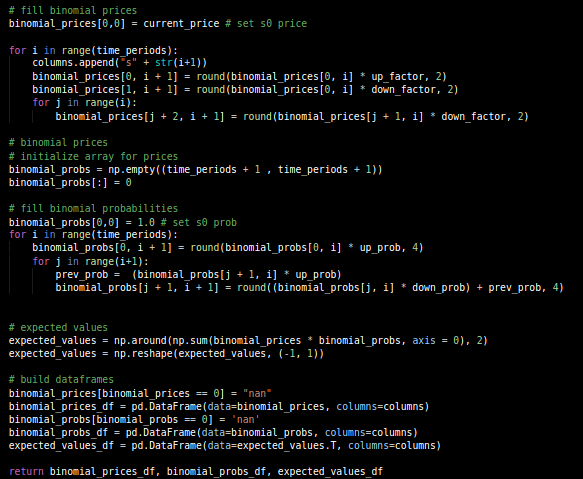
\includegraphics[scale = .55]{imgs/binomial_tree_2.png}
  \caption{Function to construct Binomial Tree part 2.}
  \label{fig:binomial_2}
\end{figure}

\begin{figure}[H]
\centering
  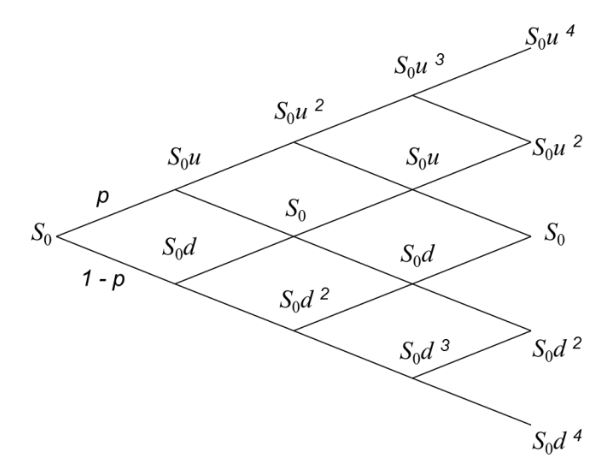
\includegraphics[scale = .75]{imgs/binomial_example.JPG}
  \caption{Visual Explanation of how the projected prices are computed. u = Up Factor and d = Down Factor}
  \label{fig:binomial_ex}
\end{figure}

\begin{table}[H]
\centering
  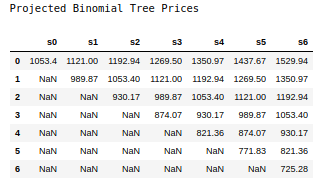
\includegraphics[scale = .90]{imgs/binomial_prices.png}
  \caption{The projected Stock Price Binomial Trees. }
  \label{tbl:binomial_prices}
\end{table}

\begin{figure}[H]
\centering
  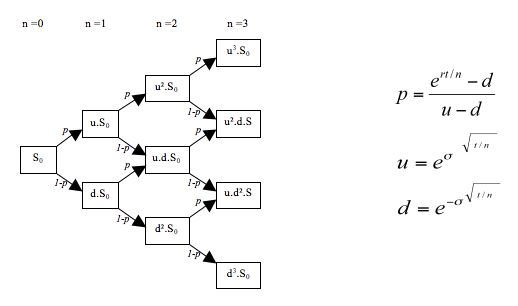
\includegraphics[scale = .75]{imgs/binomial_example_prob.JPG}
  \caption{Visual Explanation of how the projected probabilities are computed.}
  \label{fig:binomial_ex2}
\end{figure}

\begin{table}[H]
\centering
  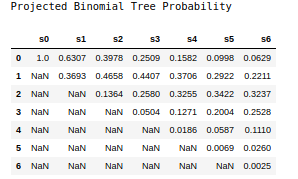
\includegraphics[scale = .90]{imgs/binomial_probs.png}
  \caption{The projected Probability Binomial Trees. }
  \label{tbl:binomial_probs}
\end{table}

\noindent
The final step was then to compute the expected values which will be shown in (iii). The expected values are computed as the sum product of each column of the two outputs described above. All the outputted numpy arrays described above were converted and returned as pandas dataframes. 

% END Question (i) ##########################################################################################################

% Question (ii) #############################################################################################################

\subsection{Q3 (ii)}\label{sssec:pt1q3ii}
\textbf{Utilizing the binomial tree from (i), what is the probability that at the end of the 6 month period
the price will be greater than the starting price.}

\noindent
The code for this task can be found in ‘Question 3 (ii)’ in the python notebook. To calculate the probability for this question we took the sum of the last column for Table.~\ref{tbl:binomial_probs} where the corresponding price is greater than the last closing price. This means $p = (0.0629 + 0.2211 + 0.3237) \times 100 $, which is equal to 60.77\%. 

% END Question (ii) #########################################################################################################

% Question (iii) ############################################################################################################

\subsection{Q3 (iii)}\label{sssec:pt1q3iii}
\textbf{Calculate the expected stock price, on a monthly basis.}

\noindent
The computation to get the stock prices on a monthly basis was described in the function which was used in (i), and these prices are shown in Table.~\ref{tbl:binomialexpectedprices}. Code for this question can be found in ‘Question 3 (iii)’ in the python notebook.

\begin{table}[H]
    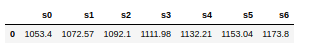
\includegraphics[width=\linewidth]{imgs/binomial_prices_monthly.png}
    \caption{Table for the expected stock prices on a monthly basis using Binomial Trees.}
    \label{tbl:binomialexpectedprices}
\end{table}

% END Question (iii) #########################################################################################################
